\documentclass{article}
\usepackage{color}
\usepackage{graphicx}
\begin{document}
\huge \textcolor{red}{PRESENTACION DE \LaTeX }

\vspace{0.5cm}

\Large PARA QUE SE UTILIZA \LaTeX?

\vspace{0.3cm}

Es un sistema de composición de textos, orientado a la creación de documentos escritos que presenten una alta calidad tipográfica. Por sus características y posibilidades, es usado de forma especialmente intensa en la generación de artículos y libros científicos que incluyen, entre otros elementos, expresiones matemáticas.

\vspace{0.5cm}

\Large \textcolor{blue}{DESCRIPCION}

LaTeX es un sistema de composición de textos que está formado mayoritariamente por órdenes construidas a partir de comandos de Tex unlenguaje de bajo nivel en el sentido de que sus acciones últimas son muy elementales pero con la ventaja añadida depoder aumentar las capacidades de LaTeX utilizando comandos propios del TeX descritos en The TeXbook Esto es lo que convierte a LaTeX en una herramienta práctica y útil pues, a su facilidad de uso, se une toda la potencia de TeX. Estas características hicieron que LaTeX se extendiese rápidamente entre un amplio sector científico y técnico, hasta el punto de convertirse en uso obligado en comunicaciones y congresos, y requerido por determinadas revistas a la hora de entregar artículos académicos.

\vspace{0.5cm}

\Large \textcolor{blue}{USO}

LaTeX presupone una filosofía de trabajo diferente a la de los procesadores de texto habituales 
y se basa en instrucciones. Tradicionalmente, este aspecto se ha considerado una desventaja (probablemente la única). Sin embargo, LaTeX, a diferencia de los procesadores de texto de tipo WYSIWYG, permite a quien escribe un documento centrarse exclusivamente en el contenido, sin tener que preocuparse de los detalles del formato. Además de sus capacidades gráficas para representar ecuaciones, fórmulas complicadas, notación científica e incluso musical, permite estructurar fácilmente el documento (con capítulos, secciones, notas, bibliografía, índices analíticos, etc.), lo cual brinda comodidad y lo hace útil para artículos académicos y libros técnicos.

\vspace{0.2cm}

Con LaTeX, la elaboración del documento requiere normalmente de dos etapas: en la primera hay que crear mediante cualquier editor de texto plano un archivo o fichero fuente que, con las órdenes y comandos adecuados, contenga el texto que queramos imprimir. La segunda etapa consiste en procesar este archivo; el procesador de textos interpreta las órdenes escritas en él y compila el documento, dejándolo preparado para que pueda ser enviado a la salida correspondiente, ya sea la pantalla o la impresora. Si se quiere añadir o cambiar algo en el documento, se deberán hacer los cambios en el archivo fuente y procesarlo de nuevo. Esta idea, que puede parecer poco práctica a priori, es conocida a los que están familiarizados con el proceso de compilación que se realiza con los lenguajes de programación de alto nivel (C, C++, etc.), ya que es completamente análogo.

\vspace{0.2cm}
El modo en que LaTeX interpreta la forma que debe tener el documento es mediante etiquetas. Por ejemplo, Documentclass {articule} le dice a LaTeX que el documento que va a procesar es un artículo. Puede resultar extraño que hoy en día se siga usando una herramienta que no sea del tipo  WYSIWYG (lo que ves es lo que obtienes), pero las características de LaTeX siguen siendo muchas y muy variadas. También hay varias herramientas o aplicaciones que ayudan a una persona a escribir estos documentos de una manera más visual (LyX, TeXmacs y otros). A estas herramientas se les llama WYSIWYM (lo que ves es lo que quieres decir).

\vspace{0.5cm}

\Large \textcolor{red}{ALGUNOS EJEMPLOS DE CODIGO}

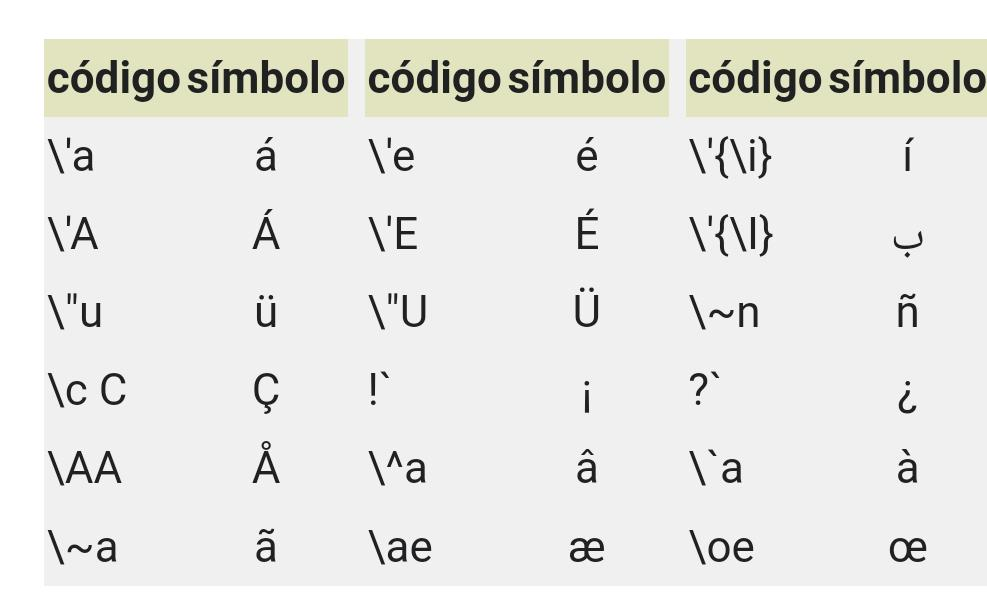
\includegraphics[scale = 0.3]{codigouno.jpg.jpeg}

\Large \textbf{Imagen 1}

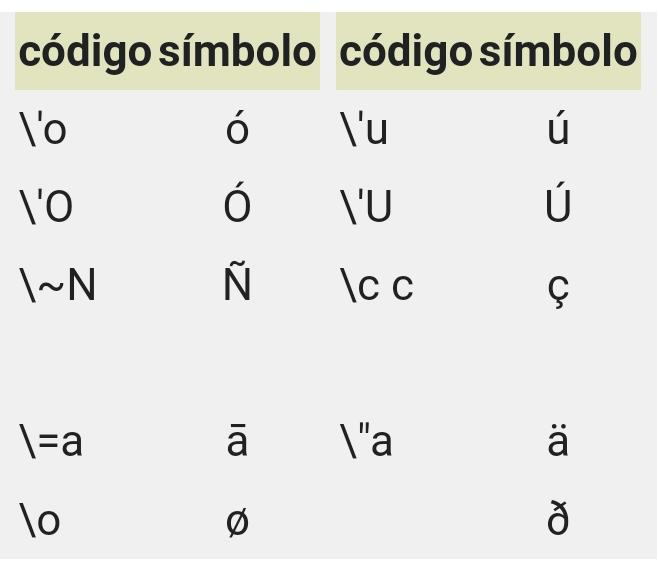
\includegraphics[scale = 0.5]{codigodos.jpg.jpeg}

\Large \textbf{Imagen 2}

\end{document}
